\documentclass[conference]{IEEEtran}
\usepackage{cite}
\usepackage{amsmath,amssymb,amsfonts}
\usepackage{algorithm}
\usepackage{algpseudocode}
\usepackage{graphicx}
\usepackage{textcomp}
\usepackage{xcolor}
\usepackage{array}
\usepackage{booktabs}
\usepackage{multirow}
\usepackage{tikz}
\usetikzlibrary{arrows.meta,positioning}
\usepackage{url}
\usepackage[hidelinks]{hyperref}

\newcolumntype{L}[1]{>{\raggedright\arraybackslash}p{#1}}
\graphicspath{{figures/}}
% Shows an image if the file exists, otherwise a labelled placeholder box (so the paper always compiles).
\newcommand{\figorbox}[2]{\IfFileExists{figures/#1}{\includegraphics[width=#2]{#1}}{\fbox{\parbox[c][2.2cm][c]{\dimexpr#2-2\fboxsep-2\fboxrule\relax}{\centering\footnotesize [\detokenize{#1} not found]}}}}
\algrenewcommand\algorithmicrequire{\textbf{Input:}}
\algrenewcommand\algorithmicensure{\textbf{Output:}}

\begin{document}

\title{Evidence-Grounded Clinical Trial Eligibility Screening with a Fine-Tuned Small Language Model: Low-Rank Adaptation, Key--Value Caching, Tiled Attention, and Speculative Decoding}

\author{\IEEEauthorblockN{Maryam Fatima}
\IEEEauthorblockA{Department of Computer Science\\
FAST National University of Computer and Emerging Sciences, Islamabad\\
maryam.faatim4@gmail.com}}

\maketitle

\begin{abstract}
Matching a patient to a clinical trial requires judging each inclusion and exclusion criterion against a free-text patient description and citing the sentences that support the judgment. This paper presents an end-to-end, reproducible system built on a small open-weight Transformer, Qwen2.5-1.5B-Instruct, fine-tuned with low-rank adaptation (LoRA) on the TrialGPT Criterion Annotations dataset using a patient-grouped split of 37 training, 8 validation, and 8 test patients. The model returns one of six expert label categories together with the identifiers of the supporting sentences. On the held-out test patients, fine-tuning raises accuracy from 0.117 to 0.743, macro-F1 from 0.142 to 0.536, and evidence F1 from 0.124 to 0.546. The dominant remaining error is treating missing information as proof that an exclusion criterion does not apply. Beyond accuracy, three inference mechanisms are implemented from scratch and validated against references. A key--value (KV) cached greedy decoder is token-identical to an uncached decoder and up to 8.0 times faster. A tiled attention with online softmax agrees with a float64 reference to within one part in a thousand in half precision and uses 125 times less memory at 4096 tokens. A greedy speculative decoder preserves the output exactly but, on a free T4 graphics processor, gives no speedup; the best measured value is 1.00 times. A browser application exposes screening, evidence inspection, report export, and a live benchmark of the decoding modes. The system is an educational prototype and not a clinical decision tool.
\end{abstract}

\begin{IEEEkeywords}
clinical trial matching, eligibility criteria, low-rank adaptation, KV cache, online softmax, speculative decoding, evidence retrieval
\end{IEEEkeywords}

%==============================================================================
\section{Introduction}
Deciding whether a patient may enter a clinical trial requires reading the patient description and checking it against every inclusion and exclusion criterion of the trial. The task is slow for clinicians and hard for automatic systems for three reasons. First, criteria are free text and often compound. Second, the patient record rarely mentions every fact that a criterion needs, so a system must be able to state that information is missing instead of guessing. Third, a decision is only useful if it points to the sentences that justify it.

Recent work has shown that large language models can perform this criterion-level matching when prompted \cite{trialgpt}, and that open models adapted with supervised data can approach proprietary ones \cite{nievas}. Those results, however, rely on large proprietary models or substantial hardware. This paper asks a practical question: how far can a 1.5-billion-parameter open-weight Transformer be taken on a free graphics processing unit (GPU) when fine-tuning, evaluation, inference acceleration, and a user-facing application must all be implemented and verified by one person?

The contributions are as follows.
\begin{itemize}
\item A LoRA-adapted Qwen2.5-1.5B-Instruct model that, given a patient note, a criterion type, and a criterion text, returns a structured label and supporting sentence identifiers. It is evaluated before and after fine-tuning on identical examples under a patient-grouped protocol.
\item An evaluation that preserves all six expert label categories, defines an explicit policy for records without evidence, and analyzes errors, with emphasis on missing information.
\item From-scratch implementations of a KV-cached decoder, tiled online-softmax attention, and greedy speculative decoding. Each is validated for exact or numerically bounded agreement with a reference and measured honestly, including a case where it does not help.
\item A browser application with per-criterion evidence, a rule-based overall outcome, report export, and a live comparison of decoding modes.
\item A reproducible package: code, split manifest, logs, and an adapter download.
\end{itemize}
Section~\ref{sec:related} reviews related work. Section~\ref{sec:methods} describes the data, model, algorithms, and application. Section~\ref{sec:setup} gives the experimental setup, Section~\ref{sec:results} presents and discusses the results, and Sections~\ref{sec:limits} and~\ref{sec:conclusion} state the limitations and conclusions.

%==============================================================================
\section{Related Work}\label{sec:related}
\textbf{Trial matching with language models.} TrialGPT \cite{trialgpt} decomposes matching into retrieval, criterion-level matching with explanations and evidence sentences, and ranking. Its criterion-level annotations by physicians form the dataset used here \cite{dataset}. Its strongest results use a proprietary model, which limits local use and reproducibility. Nievas et al.\ \cite{nievas} study the distillation of a large model into smaller open models for the same matching problem. The present work follows this direction, but fine-tunes directly on the expert labels and evidence sentences and does not use any model-generated annotation.

\textbf{Parameter-efficient adaptation.} LoRA \cite{lora} freezes the pretrained weights and learns low-rank updates, and QLoRA \cite{qlora} adds four-bit quantization of the frozen weights to reduce memory further. QLoRA is the safer choice when a model barely fits the GPU. Here the 1.5-billion-parameter model fits in half precision with LoRA, so quantization was not needed and the simpler method was used.

\textbf{Efficient attention.} Softmax over a long row can be computed in a single pass with a running maximum and normalizer \cite{onlinesoftmax}. FlashAttention \cite{flash1} and FlashAttention-2 \cite{flash2} use this idea inside fused GPU kernels that process tiles in fast on-chip memory. Their speed depends on hardware features that a free Turing-generation GPU lacks, which is why the implementation in this paper is evaluated mainly for correctness and memory.

\textbf{Efficient decoding.} Autoregressive Transformers \cite{vaswani} reuse keys and values of earlier tokens through a cache. Speculative decoding \cite{specdec,specsamp} lets a cheap draft model propose several tokens that the target model verifies in one pass. The speedup depends on the draft acceptance rate and on the cost ratio between draft and target.

Table~\ref{tab:sources} summarizes how each source informs the design and what limits its direct use.

\begin{table}[!t]
\caption{Main Sources and Their Role in This Work}
\label{tab:sources}
\centering
\footnotesize
\setlength{\tabcolsep}{3pt}
\begin{tabular}{L{0.13\columnwidth}L{0.36\columnwidth}L{0.42\columnwidth}}
\toprule
Source & Contribution & Limit for this task / use here \\
\midrule
\cite{trialgpt} & Criterion-level matching, evidence, ranking & Proprietary model; dataset source only \\
\cite{nievas} & Open models adapted for trial matching & Distilled labels; here expert labels are used \\
\cite{lora}, \cite{qlora} & Low-rank adapters; quantized variant & Quantization unnecessary; LoRA selected \\
\cite{onlinesoftmax}, \cite{flash1}, \cite{flash2} & Online softmax; fused tiled attention & Fused kernels unavailable on T4; algorithm reimplemented \\
\cite{specdec}, \cite{specsamp} & Draft-and-verify decoding & Gain depends on draft cost; measured here \\
\bottomrule
\end{tabular}
\end{table}

%==============================================================================
\section{Materials and Methods}\label{sec:methods}

\subsection{Dataset and Patient-Grouped Split}
Only the TrialGPT Criterion Annotations dataset \cite{dataset} is used. It contains 1,015 annotated patient--criterion pairs from 53 patients, labelled by three physicians \cite{trialgpt}. Each row holds a patient note with numbered sentences, a trial identifier and title, the criterion type, the criterion text, the expert eligibility label, and the identifiers of the expert-selected evidence sentences. The dataset also stores predictions and explanations produced earlier by GPT-4 and a flag that marks the dataset's own training subset. These fields were removed immediately after loading, and an assertion verifies that no column whose name begins with ``gpt4'' remains, so earlier model outputs cannot reach a prompt or an evaluation.

The split follows the common protocol. The unique patient identifiers are sorted, shuffled with the NumPy generator \texttt{default\_rng(42)}, and assigned in order: the first 37 to training, the next 8 to validation, and the remaining 8 to testing. All rows of a patient belong to exactly one split, set intersections are asserted to be empty, and the manifest with patient identifiers and counts is published. One training row has no criterion text. It was excluded after the split had been computed, logged, and counted, so the prescribed 37/8/8 partition is unchanged. The usable rows number 602, 206, and 206.

All six expert label categories are preserved (Table~\ref{tab:labels}). Inclusion criteria use \emph{included}, \emph{not included}, \emph{not enough information}, and \emph{not applicable}; exclusion criteria use \emph{excluded}, \emph{not excluded}, and the same last two. The distribution is strongly imbalanced: the label \emph{not excluded} alone covers 483 of the 1,014 usable rows, whereas \emph{excluded} has 10 and \emph{not applicable} for inclusion has 9. Accuracy alone is therefore a weak indicator, and macro-F1 and per-class scores are reported throughout. The test split contains no \emph{excluded} example.

\begin{table}[!t]
\caption{Usable Rows per Label and Split}
\label{tab:labels}
\centering
\footnotesize
\begin{tabular}{llrrr}
\toprule
Type & Label & Train & Val & Test \\
\midrule
\multirow{4}{*}{Inclusion} & included & 88 & 35 & 27 \\
 & not included & 13 & 3 & 7 \\
 & not enough information & 109 & 27 & 38 \\
 & not applicable & 5 & 1 & 3 \\
\midrule
\multirow{4}{*}{Exclusion} & excluded & 8 & 2 & 0 \\
 & not excluded & 291 & 101 & 91 \\
 & not enough information & 65 & 26 & 28 \\
 & not applicable & 23 & 11 & 12 \\
\midrule
\multicolumn{2}{l}{Total rows (patients)} & 602 (37) & 206 (8) & 206 (8) \\
\bottomrule
\end{tabular}
\end{table}

\subsection{Model Selection and Feasibility}
Table~\ref{tab:models} compares the candidates. The target is Qwen2.5-1.5B-Instruct \cite{qwen25}, a decoder-only Transformer with 1.544 billion parameters (2.88~GiB in half precision), 28 layers, hidden size 1536, 12 query heads and 2 key--value heads (grouped-query attention \cite{gqa}), head dimension 128, rotary position embeddings \cite{rope}, SwiGLU feed-forward layers, RMS normalization, tied input and output embeddings, a vocabulary of 151,936 tokens, a context window of 32,768 tokens, and the Apache~2.0 license. The draft model for speculative decoding is Qwen2.5-0.5B-Instruct (0.494 billion parameters, 0.92~GiB, 24 layers, hidden size 896, 14 query and 2 key--value heads, head dimension 64). Both models use the same tokenizer; this was verified by comparing the full vocabularies and by encoding a sample text with both.

The size of the key--value cache per token is $2\,N_\ell H_{kv} d\, b$ bytes, where $N_\ell$ is the number of layers, $H_{kv}$ the number of key--value heads, $d$ the head dimension, and $b$ the bytes per element. This gives 28,672 bytes per token for the target and 12,288 bytes for the draft in half precision. Grouped-query attention makes the target cache six times smaller than with 12 key--value heads. LoRA training of the target peaked at 7.95~GiB on a GPU with 14.56~GiB of usable memory, so the choice is feasible with margin.

\begin{table}[!t]
\caption{Candidate Open-Weight Decoder Models}
\label{tab:models}
\centering
\footnotesize
\setlength{\tabcolsep}{3pt}
\begin{tabular}{L{0.27\columnwidth}L{0.12\columnwidth}L{0.17\columnwidth}L{0.33\columnwidth}}
\toprule
Model & Params & Licence & Decision \\
\midrule
Qwen2.5-1.5B-Instruct & 1.54\,B & Apache 2.0 & Selected as target \\
Qwen2.5-0.5B-Instruct & 0.49\,B & Apache 2.0 & Selected as draft (same tokenizer) \\
Llama-3.2-1B-Instruct & $\approx$1.2\,B & Community licence, gated & Not used: gated access \\
Qwen2.5-3B-Instruct & $\approx$3.1\,B & Different licence & Not used: weights $\approx$5.8~GiB, slower training \\
\bottomrule
\end{tabular}
\end{table}

\subsection{Input, Output, and Tokenization}
A shared module builds every prompt, so that training, evaluation, and the application cannot drift apart. The system message states that this is an educational screening task, that one criterion must be judged using only the note, that missing facts must never be assumed, and that the answer must be JSON. The user message contains the numbered note sentences, the criterion type and text, the allowed labels for that type, and the required format. The output schema is a JSON object with a label and a sorted list of evidence sentence identifiers:
\begin{center}
\small\texttt{\{"label": <label>, "evidence": [ids]\}}
\end{center}
The Qwen chat template and tokenizer are used. The training target is this JSON string followed by the end-of-sequence token. A parser extracts the first JSON object and accepts it only if the label belongs to the allowed set of the criterion type; otherwise the output is marked invalid, scored as an error, and never repaired.

Prompt plus target lengths in tokens are: training mean 294, 95th percentile 460, maximum 589; validation mean 307, maximum 423; test mean 277, maximum 483. The maximum training length was set to 1,024 tokens, so no example is truncated and no evidence sentence can be removed. The training code raises an error instead of truncating silently, and the application refuses inputs above 1,536 tokens for the same reason. Because the dataset explanations are GPT-4 outputs and are excluded, the model is not trained to write explanations; the application builds them from the label and the cited sentences (Section~\ref{sec:app}).

\subsection{Fine-Tuning}
LoRA replaces a frozen weight matrix $W_0$ by
\begin{equation}
W = W_0 + \frac{\alpha}{r}\,BA, \quad B\in\mathbb{R}^{d_{\text{out}}\times r},\; A\in\mathbb{R}^{r\times d_{\text{in}}},
\label{eq:lora}
\end{equation}
where only $A$ and $B$ are trained in (\ref{eq:lora}). The training objective is token-level cross-entropy computed only on the answer tokens; prompt tokens receive the ignore label. Table~\ref{tab:train} lists the configuration. The adapters add 18,464,768 trainable parameters, 1.18\% of the total. Half-precision automatic mixed precision with a gradient scaler was used because the GPU has no bfloat16 support, with the trainable weights kept in single precision. Gradient checkpointing and a micro-batch of one example with 16 accumulation steps were adopted after out-of-memory errors with micro-batches of four and two. One checkpoint is saved per epoch and the epoch is chosen by validation macro-F1, not by loss. At inference the adapter is merged into the base weights. No hyperparameter search was performed.

\begin{table}[!t]
\caption{Fine-Tuning Configuration}
\label{tab:train}
\centering
\footnotesize
\begin{tabular}{L{0.34\columnwidth}L{0.52\columnwidth}}
\toprule
Setting & Value \\
\midrule
LoRA rank $r$ / scale $\alpha$ / dropout & 16 / 32 / 0.05 \\
Adapted modules & \texttt{q,k,v,o,gate,up,down} projections \\
Optimizer / weight decay & AdamW / 0 \\
Learning rate / schedule & $2\times10^{-4}$ / cosine, 10\% warm-up (11 steps) \\
Epochs / optimizer steps & 3 / 114 (38 per epoch) \\
Effective batch size & 16 (micro-batch 1 $\times$ 16 accumulation) \\
Gradient clipping & 1.0 \\
Precision & fp16 autocast, fp32 adapter weights \\
Maximum length / seed & 1,024 tokens / 42 \\
\bottomrule
\end{tabular}
\end{table}

\subsection{Evaluation Protocol}
Classification is evaluated with accuracy, macro-F1, per-class precision, recall, and F1, and confusion matrices, overall and separately for inclusion and exclusion criteria. Macro-F1 averages over the labels that occur in the gold labels or in the predictions, so a label predicted although absent from the gold standard lowers the score; the variant restricted to gold labels is also stored. Invalid outputs are counted as errors and shown in a separate confusion-matrix column.

Evidence is evaluated on sets of sentence identifiers per row. With $\mathrm{TP}$, $\mathrm{FP}$, and $\mathrm{FN}$ pooled over rows,
\begin{equation}
P_{\text{micro}}=\frac{\mathrm{TP}}{\mathrm{TP}+\mathrm{FP}},\quad R_{\text{micro}}=\frac{\mathrm{TP}}{\mathrm{TP}+\mathrm{FN}},
\label{eq:prf}
\end{equation}
in (\ref{eq:prf}), and $F_1$ is the harmonic mean of the two. The policy for empty sets is explicit. A row with no gold and no predicted evidence adds nothing to the pooled counts; a row with no gold evidence but a predicted sentence adds false positives. The macro score over rows with at least one gold sentence gives zero to an empty prediction. A second macro score over all rows gives one to a correct abstention and zero to a spurious citation, and the abstention rate and false-evidence rate on rows without gold evidence are reported directly. The absence of evidence is never treated as proof: \emph{not enough information} is a separate label.

All model comparisons use greedy decoding with repetition penalty 1.0 (the model default of 1.05 would change greedy outputs), at most 64 new tokens, and half precision. The base and fine-tuned models receive identical prompts. The test split is blocked in the evaluation script unless a flag is passed, and it was evaluated once, after the epoch had been chosen on validation data.

\subsection{KV-Cached Autoregressive Decoding}
The decoder calls the model's forward pass with explicit cache management rather than relying on a library switch (Algorithm~\ref{alg:kv}). The prompt is processed once (prefill) with positions $0,\dots,L-1$. Afterward only the newest token is fed.

\emph{Positions.} Rotary embeddings \cite{rope} rotate keys and queries by their absolute position, and keys are stored in the cache already rotated. The new token must therefore be given the position equal to the number of cached tokens; a wrong position gives wrong outputs although all shapes still match.

\emph{Masking.} Prefill needs a causal mask. A single new query attends to all cached keys and to itself, so its attention mask is all ones over $n{+}1$ keys; no future token exists yet.

\emph{Cache growth.} The cache grows by exactly one token per step. The code counts the cached length independently and asserts that the cache length equals the count after every step. For 1,152 tokens the cache occupies $1152\times 28{,}672$ bytes, about 31.5~MiB.

\emph{Numerical differences.} The cached path multiplies one row at a time and the uncached path multiplies all rows together, so the accumulation order differs. In half precision this produces small logit differences, which change the greedy token only when the two best logits are almost tied. The uncached reference re-runs the whole sequence at every step with the cache disabled.

\begin{algorithm}[!t]
\caption{Greedy decoding with an explicit KV cache}
\label{alg:kv}
\small
\begin{algorithmic}[1]
\Require prompt $x_{1:L}$, maximum new tokens $T$, end token
\State $\ell,\mathcal{C} \gets \textsc{Forward}(x_{1:L},\ \text{positions } 0..L{-}1)$ \Comment{prefill}
\State $y_1\gets\arg\max\ell$;\ \ $n\gets L$
\For{$t=2,\dots,T$ \textbf{while} $y_{t-1}\neq$ end token}
  \State $\ell,\mathcal{C}\gets\textsc{Forward}(y_{t-1},\ \text{position } n,\ \mathcal{C})$
  \State $n\gets n+1$;\ \ \textbf{assert} $|\mathcal{C}|=n$
  \State $y_t\gets\arg\max\ell$
\EndFor
\State \Return $y_{1:t}$
\end{algorithmic}
\end{algorithm}

\subsection{Tiled Attention with Online Softmax}
Scaled dot-product attention for queries $Q$, keys $K$, and values $V$ with head dimension $d$ is
\begin{equation}
\mathrm{Attn}(Q,K,V)=\mathrm{softmax}\!\left(\frac{QK^{\top}}{\sqrt{d}}+M\right)V,
\label{eq:attn}
\end{equation}
where, in (\ref{eq:attn}), $M$ is zero for visible positions and $-\infty$ for masked ones. The reference implementation builds the full score matrix, subtracts the row maximum before exponentiation for numerical stability, and normalizes.

The tiled version processes one block of queries at a time and loops over blocks of keys, keeping for every query row a running maximum $m$, a running normalizer $\ell$, and a running weighted sum $O$. For key block $j$ with scores $S_j$,
\begin{align}
m' &= \max\!\big(m,\ \mathrm{rowmax}(S_j)\big), \label{eq:m}\\
P_j &= \exp(S_j - m'), \qquad \gamma = \exp(m - m'), \label{eq:p}\\
\ell &\leftarrow \gamma\,\ell + \mathrm{rowsum}(P_j), \quad O \leftarrow \gamma\,O + P_jV_j, \quad m\leftarrow m'. \label{eq:o}
\end{align}
After the last block the output is $O/\ell$. The factor $\gamma$ in (\ref{eq:p}) rescales everything accumulated so far to the new maximum, so the result equals the ordinary softmax up to rounding. Only one tile of scores exists at a time, which reduces the score memory from $O(L_qL_k)$ to $O(B_qB_k)$ for block sizes $B_q$ and $B_k$ (Algorithm~\ref{alg:tile}).

For causal attention the queries are taken to be the last $L_q$ positions of the $L_k$ keys, so that $L_q=1$ reproduces one cached decoding step. Key blocks entirely in the future of a query block are skipped, and blocks that touch the diagonal are masked inside the tile. A row that is fully masked in a block would give $-\infty-(-\infty)$; a safe maximum of zero is used for such rows. Half-precision inputs are accumulated in single precision, as in fused kernels.

\begin{algorithm}[!t]
\caption{Tiled attention with online softmax}
\label{alg:tile}
\small
\begin{algorithmic}[1]
\Require $Q, K, V$, block sizes $B_q, B_k$, causal flag
\For{each query block $Q_i$}
  \State $m\gets-\infty;\ \ell\gets 0;\ O\gets 0$
  \For{each key block $K_j,V_j$ \textbf{not} entirely in the future}
    \State $S\gets Q_iK_j^{\top}/\sqrt{d}$; mask diagonal blocks if causal
    \State update $m,\ell,O$ with (\ref{eq:m})--(\ref{eq:o})
  \EndFor
  \State output block $\gets O/\ell$
\EndFor
\end{algorithmic}
\end{algorithm}

\subsection{Greedy Speculative Decoding}
In each round (Algorithm~\ref{alg:spec}) the draft model proposes $k$ tokens greedily using its own cache. The target model then processes the last committed token and the $k$ drafts in a single forward pass and yields its own greedy choice $g_0,\dots,g_k$ after each input position. The longest prefix of drafts that equals the target's choices is accepted, and the target's next choice is appended: a correction when a draft was rejected, or a free bonus token when all $k$ were accepted. Every committed token is therefore the target's greedy token given the committed prefix, so the output is identical to ordinary greedy decoding; the draft only influences speed.

Cache synchronization is the delicate part. Both caches contain rejected tokens after verification and are cropped. The invariant is that the target cache holds all committed tokens except the last one, and the draft cache holds the committed tokens plus the accepted drafts that it has already processed. The draft model never feeds its last proposal, so its cache is cropped to the old committed length plus $\min(a,k-1)$. Assertions check both lengths in every round. A simple cost model describes the expected speedup. If $\tau$ is the mean number of tokens committed per round and $c$ the cost of one draft step relative to one target step, then
\begin{equation}
S \approx \frac{\tau}{1+kc},
\label{eq:cost}
\end{equation}
ignoring prefill and cache cropping.

\begin{algorithm}[!t]
\caption{One round of greedy speculative decoding}
\label{alg:spec}
\small
\begin{algorithmic}[1]
\Require committed tokens $c$, draft length $k$
\State draft proposes $d_1,\dots,d_k$ greedily (own cache)
\State target forward on $[c_{\text{last}},d_1,\dots,d_k]$ gives $g_0,\dots,g_k$
\State $a\gets$ largest $a\le k$ with $d_j=g_{j-1}$ for all $j\le a$
\State commit $d_1,\dots,d_a$ and $g_a$ (correction if $a<k$, bonus if $a=k$)
\State crop target cache to $|c_{\text{new}}|-1$ tokens
\State crop draft cache to $|c_{\text{old}}|+\min(a,k-1)$ tokens
\end{algorithmic}
\end{algorithm}

\subsection{Application}\label{sec:app}
Fig.~\ref{fig:pipeline} shows the workflow of the browser application, which is built with Gradio \cite{gradio} and the Transformers library \cite{transformers}. The user pastes a patient note, either with numbered sentences or as free text, and enters criteria under ``Inclusion criteria'' and ``Exclusion criteria'' headings, or loads an example. The sentences are numbered from zero, as in the training data. For each criterion the engine builds the prompt, decodes with the selected mode (KV cache, no cache, or speculative), parses the answer, and removes cited identifiers that do not exist in the note.

The explanation of a criterion is assembled only from the predicted label and the cited sentences; no free text is generated. For example, a label \emph{not excluded} without a cited sentence is explained as meaning that nothing in the note triggers the exclusion, not that the note proves its absence.

The overall outcome is an explicit aggregation of criterion-level decisions, not a labelled ground truth, because the dataset only provides criterion-level labels. A criterion \emph{fails} if an inclusion criterion is \emph{not included} or an exclusion criterion is \emph{excluded}; it is \emph{unresolved} if the label is \emph{not enough information} or the answer is invalid; it \emph{passes} otherwise, except that \emph{not applicable} is neutral. If any criterion fails, the outcome is ``likely not eligible''. Otherwise, if any is unresolved, it is ``more information needed'', and the unresolved criteria are listed. Otherwise, if at least one passes, it is ``likely eligible''.

The report is saved as HTML and Markdown and contains the disclaimer, the outcome, a criterion table, the cited evidence text, the explanations, the raw model outputs, and provenance (model, adapter and its source, device, precision, decoding mode, and a fingerprint of the inputs). A benchmark tab runs the same prompts through all three decoding modes after a warm-up pass and reports time, tokens per second, peak memory on a GPU, token equality with the no-cache reference, draft acceptance, and speedups. Saved experiment tables are read from the repository files. Inputs are validated (empty note, missing type headings, excessive length, too many criteria), and model errors are reported as messages without ending the session. The page shows the notice that the system is an educational screening prototype and not a clinical enrollment decision. The application starts with \texttt{python app.py}, detects a GPU automatically, runs on the CPU otherwise, and downloads the adapter from the release page if it is not present.

\begin{figure*}[!t]
\centering
\resizebox{0.95\textwidth}{!}{%
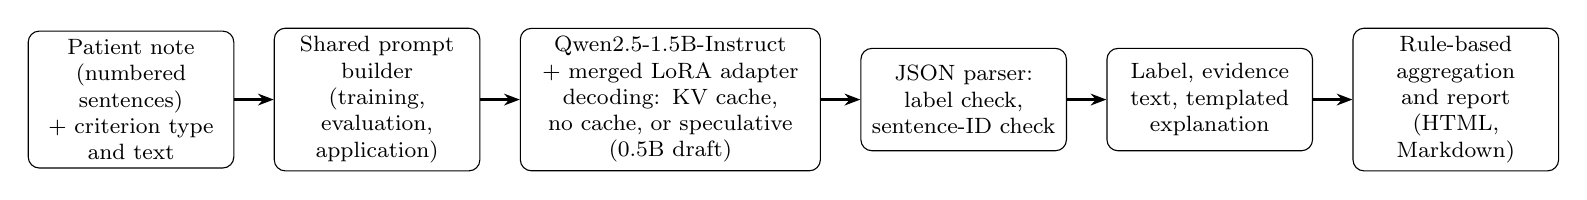
\begin{tikzpicture}[node distance=5mm,
 box/.style={draw, rounded corners, align=center, font=\footnotesize, minimum height=13mm, text width=24mm, inner sep=3pt},
 arr/.style={-{Stealth[length=2mm]}, thick}]
\node[box] (in) {Patient note\\(numbered sentences)\\+ criterion type\\and text};
\node[box, right=of in] (pr) {Shared prompt\\builder\\(training, evaluation,\\application)};
\node[box, right=of pr, text width=36mm] (m) {Qwen2.5-1.5B-Instruct\\+ merged LoRA adapter\\decoding: KV cache,\\no cache, or speculative\\(0.5B draft)};
\node[box, right=of m] (pa) {JSON parser:\\label check,\\sentence-ID check};
\node[box, right=of pa] (ex) {Label, evidence\\text, templated\\explanation};
\node[box, right=of ex] (ag) {Rule-based\\aggregation\\and report\\(HTML, Markdown)};
\draw[arr] (in)--(pr); \draw[arr] (pr)--(m); \draw[arr] (m)--(pa); \draw[arr] (pa)--(ex); \draw[arr] (ex)--(ag);
\end{tikzpicture}}
\caption{Architecture of the screening system. The same prompt builder is used for training, evaluation, and the browser application; invalid model outputs are marked unresolved and are never repaired.}
\label{fig:pipeline}
\end{figure*}

%==============================================================================
\section{Experimental Setup and Metrics}\label{sec:setup}
\textbf{Hardware and software.} All training and measurements ran on a free Kaggle notebook with one NVIDIA Tesla T4 GPU (14.56~GiB usable memory, compute capability 7.5, no bfloat16 and no FlashAttention kernels) and Python 3.13. PyTorch, Transformers \cite{transformers}, and PEFT versions are those of the Kaggle image at the time of the runs. No paid service was used. The application was also run on a personal computer.

\textbf{Training and evaluation.} Training used the configuration of Table~\ref{tab:train} with seed 42; a repeated run reproduced the validation losses exactly, which shows that training is deterministic. The evaluation used batches of 16 prompts sorted by length.

\textbf{KV-cache experiments.} Correctness compares cached and uncached greedy tokens for four synthetic lengths (input/output of 64/32, 256/64, 512/128, and 1024/128 tokens) and for 30 real validation prompts, in half and single precision, and measures the largest absolute logit difference by teacher forcing. The benchmark covers six input/output length pairs with batch size one, a warm-up run, three repetitions, and synchronized timing. Peak memory is the maximum allocated memory above the loaded weights.

\textbf{Attention experiments.} Eight shape and mask cases (tiny, divisible and non-divisible lengths, queries shorter than keys, non-causal, a single query, large scores, and a model-sized case with 12 heads and head dimension 128) are evaluated in float64, float32, and float16 against a float64 reference. The tolerances are $10^{-9}$, $10^{-4}$, and $10^{-2}$. A hand-sized example checks causality, and a stability demonstration uses scores up to 211. The speed benchmark uses half precision, causal masking, 12 heads, head dimension 128, lengths from 256 to 4096, one warm-up call, and the median of five synchronized runs.

\textbf{Speculative-decoding experiments.} Two workloads are used. Workload A consists of 40 real validation prompts (stop at the end token, at most 64 new tokens). Workload B consists of two synthetic prompts of 256 and 768 tokens with exactly 96 new tokens. Draft lengths $k\in\{2,3,4,6\}$ and three drafts are compared: the target itself (an oracle control), the base 0.5B model, and the LoRA-fine-tuned 0.5B model. The draft was fine-tuned with the recipe of Table~\ref{tab:train} (8,798,208 trainable parameters, validation loss 0.1495, 0.1333, and 0.1396 for the three epochs). Every configuration is compared token by token with ordinary cached greedy decoding, with two repetitions in half precision and one in single precision. The assisted-generation function of the Transformers library is run as an independent reference at $k=4$.

\textbf{Reproducibility.} Code, split manifest, logs, and scripts are in the repository \url{https://github.com/Maryam-Faatima/clinical_trial_matching_llm}. The adapter is available at \url{https://github.com/Maryam-Faatima/clinical_trial_matching_llm/releases/download/v1.0/adapter_epoch_3.zip}. A recorded demonstration is at \url{VIDEO-LINK-HERE}.

%==============================================================================
\section{Results and Discussion}\label{sec:results}

\subsection{Fine-Tuning and Epoch Selection}
Fig.~\ref{fig:curves} shows the training and validation losses. The loss accumulated over 16 examples falls from about 0.10--0.17 in the first epoch to 0.03--0.08 in the third, while the validation loss stays between 0.1255 and 0.1327 and is lowest after epoch 2. Training took 834~s with a peak memory of 7.95~GiB. Table~\ref{tab:val} shows that the validation macro-F1 nevertheless increases at every epoch (0.353, 0.444, 0.574), whereas the lowest loss occurs at epoch 2. Loss and macro-F1 measure different things; loss is dominated by the frequent labels, and macro-F1 rewards the rare ones. Epoch 3 was selected because macro-F1 is the metric of interest. The validation set contains only two \emph{excluded} and three \emph{not included} examples, so this selection is noisy, which is noted in Section~\ref{sec:limits}.

\begin{figure}[!t]
\centering
\figorbox{training_curves.png}{\columnwidth}
\caption{Training loss per optimizer step and validation loss per epoch for the LoRA fine-tuning of Qwen2.5-1.5B-Instruct.}
\label{fig:curves}
\end{figure}

\begin{table}[!t]
\caption{Validation Results Before and After Fine-Tuning ($n=206$)}
\label{tab:val}
\centering
\footnotesize
\setlength{\tabcolsep}{3pt}
\begin{tabular}{lcccc}
\toprule
Model & Val. loss & Acc. & Macro-F1 & Evid. micro-F1 \\
\midrule
Base (no adaptation) & -- & 0.107 & 0.118 & 0.128 \\
Epoch 1 & 0.1327 & 0.728 & 0.353 & 0.459 \\
Epoch 2 & 0.1255 & 0.752 & 0.444 & 0.541 \\
Epoch 3 (selected) & 0.1300 & 0.767 & 0.574 & 0.558 \\
\bottomrule
\end{tabular}
\end{table}

\subsection{Held-Out Test Results}
Table~\ref{tab:test} gives the test results and Fig.~\ref{fig:beforeafter} visualizes the change. Fine-tuning raises overall accuracy from 0.117 to 0.743 and macro-F1 from 0.142 to 0.536. A classifier that always answers \emph{not excluded} would reach an accuracy of 0.442 (91 of 206), so the fine-tuned model is well above this baseline. Compared with validation (0.767 accuracy, 0.574 macro-F1), the test scores are slightly lower, which gives no sign that the epoch selection overfitted the validation patients. Macro-F1 is computed over the five labels that occur in the test gold labels or predictions; the test set has no \emph{excluded} row and the fine-tuned model never predicts that label. The base model predicts \emph{excluded} 84 times, always wrongly, so its macro-F1 is 0.142 over six labels and 0.171 when restricted to the gold labels.

Inclusion criteria are easier (accuracy 0.800) than exclusion criteria (0.710), but the macro-F1 values are low for both (0.433 and 0.400) because several labels are never predicted correctly. Table~\ref{tab:perclass} and Table~\ref{tab:conf} show where the errors are. The labels \emph{included} (F1 0.898) and \emph{not excluded} (F1 0.826) are handled well. The label \emph{not enough information} reaches an F1 of 0.639 overall, with a recall of 1.000 for inclusion criteria but 0.000 for exclusion criteria. \emph{Not included} (0 of 7) and \emph{not applicable} (3 of 15) are largely missed.

Fig.~\ref{fig:conf} contrasts the confusion matrices of the base and fine-tuned models. The base model is format-compliant (no invalid outputs) but misreads the label semantics: of the 91 \emph{not excluded} rows it answers \emph{excluded} 57 times and \emph{not applicable} 33 times, and it never predicts \emph{not enough information}. This behavior is the reason for supervised adaptation. The fine-tuned model confuses the same rare classes in a different way, by collapsing them into the majority decisions.

\begin{table}[!t]
\caption{Test Results ($n=206$; Inclusion $n=75$, Exclusion $n=131$)}
\label{tab:test}
\centering
\footnotesize
\setlength{\tabcolsep}{3pt}
\begin{tabular}{llccccc}
\toprule
Model & Subset & Acc. & Macro-F1 & \multicolumn{3}{c}{Evidence micro} \\
\cmidrule(lr){5-7}
 & & & & P & R & F1 \\
\midrule
Base & Overall & 0.117 & 0.142 & 0.075 & 0.362 & 0.124 \\
Fine-tuned & Overall & 0.743 & 0.536 & 0.530 & 0.564 & 0.546 \\
Base & Inclusion & 0.227 & 0.195 & 0.323 & 0.339 & 0.331 \\
Fine-tuned & Inclusion & 0.800 & 0.433 & 0.588 & 0.758 & 0.662 \\
Base & Exclusion & 0.053 & 0.057 & 0.033 & 0.406 & 0.062 \\
Fine-tuned & Exclusion & 0.710 & 0.400 & 0.300 & 0.188 & 0.231 \\
\bottomrule
\end{tabular}
\end{table}

\begin{figure*}[!t]
\centering
\figorbox{before_after_test.png}{0.85\textwidth}
\caption{Accuracy, macro-F1, and evidence micro-F1 of the base and fine-tuned models on the test split, overall and for inclusion and exclusion criteria.}
\label{fig:beforeafter}
\end{figure*}

\begin{table}[!t]
\caption{Per-Class Results of the Fine-Tuned Model on the Test Split}
\label{tab:perclass}
\centering
\footnotesize
\begin{tabular}{lcccc}
\toprule
Label & Precision & Recall & F1 & Support \\
\midrule
included & 1.000 & 0.815 & 0.898 & 27 \\
not included & 0.000 & 0.000 & 0.000 & 7 \\
not enough information & 0.717 & 0.576 & 0.639 & 66 \\
not applicable & 0.750 & 0.200 & 0.316 & 15 \\
not excluded & 0.709 & 0.989 & 0.826 & 91 \\
excluded & -- & -- & -- & 0 \\
\bottomrule
\end{tabular}
\end{table}

\begin{table}[!t]
\caption{Confusion Matrix of the Fine-Tuned Model on the Test Split (Rows: Gold, Columns: Predicted). Abbreviations: inc.\ = included, n.inc.\ = not included, NEI = not enough information, N/A = not applicable, n.exc.\ = not excluded.}
\label{tab:conf}
\centering
\footnotesize
\begin{tabular}{lccccc}
\toprule
Gold $\backslash$ Pred. & inc. & n.inc. & NEI & N/A & n.exc. \\
\midrule
included & 22 & 0 & 5 & 0 & 0 \\
not included & 0 & 0 & 7 & 0 & 0 \\
NEI & 0 & 0 & 38 & 0 & 28 \\
N/A & 0 & 0 & 3 & 3 & 9 \\
not excluded & 0 & 0 & 0 & 1 & 90 \\
\bottomrule
\end{tabular}
\end{table}

\begin{figure*}[!t]
\centering
\figorbox{confusion_test.png}{0.9\textwidth}
\caption{Confusion matrices on the test split for the base model (top row) and the fine-tuned model (bottom row): overall, inclusion criteria, and exclusion criteria. Rows are gold labels and columns are predictions.}
\label{fig:conf}
\end{figure*}

\subsection{Evidence Localization}
The pooled evidence precision, recall, and F1 of the fine-tuned model are 0.530, 0.564, and 0.546 (Table~\ref{tab:test}), against 0.075, 0.362, and 0.124 for the base model. The macro F1 over rows with gold evidence is 0.581 (base 0.157), and over all rows it is 0.798 (base 0.376). On rows without gold evidence the fine-tuned model correctly cites nothing in 89.0\% of cases, whereas the base model does so in 46.9\%. Evidence for inclusion criteria (micro-F1 0.662) is much better than for exclusion criteria (0.231). The comparison of identifier sets is strict: a cited sentence that overlaps in content with a gold sentence but has a different identifier counts as an error, so these values are lower bounds on the usefulness of the citations.

\subsection{Error Analysis}
There are 53 label errors on the test split. Table~\ref{tab:errtypes} groups them, and in addition 37 rows have the correct label but a different evidence set. Table~\ref{tab:cases} lists twelve representative cases, three per category, drawn with a fixed random seed from the errors of the fine-tuned model.

\emph{Missing information treated as proof} (28 cases) is the dominant failure. For exclusion criteria with gold label \emph{not enough information}, the model returned \emph{not excluded} in all 28 cases without citing a sentence (cases 4 to 6): the note gives no information on MRI metal screening, on recent immunosuppressive treatment, or on cyclophosphamide, and the model read this silence as a negative answer. This is exactly the error that the task warns against, and it is a consequence of the class imbalance (483 of 658 exclusion rows are \emph{not excluded}) and of the small training set.

\emph{False insufficient information} (15 cases) is the opposite, conservative error. In case 1 the expert accepted a consent-and-compliance sentence as evidence of the ability to take oral medication, whereas the model abstained. In cases 2 and 3 the experts judged the procedure criteria as not met without citing any sentence, and the model abstained instead of answering \emph{not included}.

\emph{Not-applicable confusion} (10 cases) arises when a criterion does not concern the patient, such as pregnancy (case 7) or a tonsillectomy (case 9) in the same patient; the model answered \emph{not excluded} instead of recognizing that the criterion is not applicable.

\emph{Right label, different evidence} (37 cases) shows spurious or excessive citation. In case 10 the model cited an allergic-rhinitis sentence for a skin-test criterion that experts judged to have no evidence. In case 11 it cited the gold sentence plus one additional sentence. In case 12 it cited three symptom sentences for an exclusion criterion that experts judged as not excluded without evidence. No error of the type \emph{wrong decision polarity} occurred on the test split. On the validation split the same categories appear (45, 26, 14, 6, and 2 cases for evidence, missing information, false abstention, not-applicable confusion, and polarity), so the pattern is stable.

\begin{table}[!t]
\caption{Errors of the Fine-Tuned Model on the Test Split by Type}
\label{tab:errtypes}
\centering
\footnotesize
\begin{tabular}{lr}
\toprule
Error type & Count \\
\midrule
Missing information treated as proof & 28 \\
False \emph{not enough information} & 15 \\
Not-applicable confusion & 10 \\
Wrong decision polarity & 0 \\
\midrule
Label errors in total & 53 \\
Correct label, different evidence set & 37 \\
\bottomrule
\end{tabular}
\end{table}

\begin{table*}[!t]
\caption{Twelve Test Errors of the Fine-Tuned Model (Annotation Identifier, Criterion Type, Gold and Predicted Label)}
\label{tab:cases}
\centering
\footnotesize
\setlength{\tabcolsep}{4pt}
\begin{tabular}{rllL{0.30\textwidth}L{0.14\textwidth}L{0.14\textwidth}}
\toprule
No. & ID & Type & Criterion (shortened) & Gold & Predicted \\
\midrule
1 & 385 & incl. & Ability to take and retain oral medication & included & not enough info. \\
2 & 162 & incl. & Open abdominal aortic aneurysm repair & not included & not enough info. \\
3 & 161 & incl. & Elective carotid endarterectomy & not included & not enough info. \\
4 & 418 & excl. & Failure to pass MRI metal screening & not enough info. & not excluded \\
5 & 393 & excl. & Anti-rheumatic or immunosuppressive drugs within 3 months & not enough info. & not excluded \\
6 & 392 & excl. & Intravenous cyclophosphamide within 6 months & not enough info. & not excluded \\
7 & 697 & excl. & Pregnant & not applicable & not excluded \\
8 & 693 & excl. & Suspected sleep disorder other than sleep apnea & not applicable & not excluded \\
9 & 683 & excl. & Previous tonsillectomy & not applicable & not excluded \\
10 & 840 & incl. & Negative allergy skin test & not enough info. (evidence differs) & same label, cites sentence 1 \\
11 & 307 & incl. & Liver-damage patient selection (long text) & not enough info. (evidence differs) & same label, cites sentences 3 and 4 \\
12 & 769 & excl. & Infection of the deep upper-airway tissues & not excluded (evidence differs) & same label, cites sentences 0 to 2 \\
\bottomrule
\end{tabular}
\end{table*}

\subsection{KV-Cached Decoding}\label{sec:kvres}
\emph{Correctness.} Cached and uncached greedy decoding produced identical tokens in all four synthetic cases and in all 30 real validation prompts, in half and in single precision, so no mismatch had to be investigated. The largest absolute logit difference between the two paths is between 0.040 and 0.056 in half precision and between $1\times10^{-4}$ and $2\times10^{-4}$ in single precision. The reduction by a factor of about 300 shows that the differences are rounding noise and not a logic error in the cache.

\emph{Speed and memory.} Table~\ref{tab:kv} and Fig.~\ref{fig:kv} show that cached decoding runs at about 22--26 tokens per second at every length, at about 39~ms per generated token, whereas the uncached speed falls from 22.9 to 3.1 tokens per second as the sequence grows. The speedup therefore rises from 1.1 to 8.0 times. The uncached cost per step grows with the sequence length, and the cached cost does not at these lengths. The constant 39~ms per token indicates that single-sequence decoding on this GPU is dominated by kernel-launch and software overhead, not by arithmetic. Peak memory is similar for both paths (10--188~MiB above the weights) and is dominated by the activations of the largest forward pass; the cache itself is only about 31.5~MiB at 1,152 tokens. The cache saves time, not memory. Prefill time grows with the prompt from 46 to 275~ms.

\begin{table*}[!t]
\caption{KV-Cached Versus Uncached Greedy Decoding (Tesla T4, Half Precision, Batch Size 1; Tokens Identical in All Rows)}
\label{tab:kv}
\centering
\footnotesize
\begin{tabular}{lrrrrrr}
\toprule
Input + output tokens & Uncached tok/s & Cached tok/s & Speedup & Prefill (ms) & Decode (ms/token) & Peak MiB (unc./cached) \\
\midrule
128 + 32 & 22.9 & 25.7 & 1.1$\times$ & 46 & 38.7 & 10 / 12 \\
128 + 128 & 20.1 & 25.8 & 1.3$\times$ & 47 & 38.8 & 18 / 13 \\
512 + 32 & 6.9 & 24.3 & 3.5$\times$ & 113 & 38.9 & 54 / 62 \\
512 + 128 & 6.6 & 25.3 & 3.8$\times$ & 115 & 39.0 & 69 / 62 \\
1024 + 32 & 3.3 & 21.6 & 6.6$\times$ & 275 & 38.9 & 161 / 180 \\
1024 + 128 & 3.1 & 24.7 & 8.0$\times$ & 274 & 38.6 & 188 / 180 \\
\bottomrule
\end{tabular}
\end{table*}

\begin{figure*}[!t]
\centering
\figorbox{kv_benchmark.png}{0.8\textwidth}
\caption{Throughput (left, logarithmic axis) and peak extra memory (right) of uncached and KV-cached greedy decoding for the six length configurations.}
\label{fig:kv}
\end{figure*}

\subsection{Tiled Attention}
All 24 correctness tests (eight cases in three precisions) passed (Table~\ref{tab:attnerr}). The hand-sized example gives identical output rows for the reference and the tiled implementation, the first row equals the first value vector, and changing the last token does not change any earlier output, which confirms causality. In the stability demonstration with scores up to 211, a softmax without maximum subtraction produced non-finite values, whereas the tiled implementation stayed finite with a maximum error of $7.3\times10^{-6}$ against float64. In half precision the error of about $10^{-3}$ is mostly the rounding of the final output to 16 bits, and the reference and tiled versions are equally accurate.

Table~\ref{tab:attnbench} and Fig.~\ref{fig:attn} report speed and memory. The memory of the reference grows by about four times when the length doubles (2352~MiB at 4096 tokens), reflecting the quadratic score matrix. The tiled version needs only 18.8~MiB at 4096 tokens, 125 times less, with only a slow increase. It is, however, about 2.9 times slower than the reference and about 55 times slower than the fused memory-efficient backend of PyTorch (191 against 3.5~ms). The educational implementation is a Python loop with hundreds of block iterations, each launching about ten small GPU operations whose intermediate tiles pass through global memory. A fused kernel runs the whole loop in one launch and keeps the tiles in on-chip memory. The FlashAttention backend was unavailable because it requires compute capability 8.0 or higher, whereas the T4 has 7.5. The tiling therefore saves memory, but only fusion saves time.

\begin{table}[!t]
\caption{Absolute Error of Tiled Attention Against a Float64 Reference (Range over Eight Cases)}
\label{tab:attnerr}
\centering
\scriptsize
\setlength{\tabcolsep}{2pt}
\begin{tabular}{lccc}
\toprule
Precision & Tolerance & Max error & Mean error \\
\midrule
float64 & $10^{-9}$ & $1.1\times10^{-16}$--$4.4\times10^{-15}$ & $2.3\times10^{-17}$--$2.3\times10^{-16}$ \\
float32 & $10^{-4}$ & $1.4\times10^{-8}$--$1.3\times10^{-5}$ & $5.8\times10^{-9}$--$3.7\times10^{-7}$ \\
float16 & $10^{-2}$ & $6.0\times10^{-5}$--$9.7\times10^{-4}$ & $1.3\times10^{-5}$--$1.1\times10^{-4}$ \\
\bottomrule
\end{tabular}
\end{table}

\begin{table*}[!t]
\caption{Attention Speed and Memory (Tesla T4, Half Precision, Causal, 12 Heads, Head Dimension 128; Time in ms, Extra Memory in MiB)}
\label{tab:attnbench}
\centering
\footnotesize
\begin{tabular}{rrrrrrrr}
\toprule
Length & Reference ms & Reference MiB & Tiled ms & Tiled MiB & SDPA math ms & SDPA mem-eff. ms & SDPA mem-eff. MiB \\
\midrule
256 & 0.59 & 12.0 & 1.61 & 7.5 & 0.62 & 0.09 & 0.8 \\
512 & 1.28 & 42.0 & 4.51 & 8.3 & 1.07 & 0.14 & 1.5 \\
1024 & 4.44 & 156.0 & 14.70 & 9.8 & 3.66 & 0.33 & 3.0 \\
2048 & 16.87 & 600.1 & 51.13 & 12.8 & 13.91 & 1.12 & 6.0 \\
4096 & 66.97 & 2352.2 & 191.28 & 18.8 & 55.25 & 3.48 & 12.0 \\
\bottomrule
\end{tabular}
\end{table*}

\begin{figure*}[!t]
\centering
\figorbox{attention_benchmark.png}{0.8\textwidth}
\caption{Time (left) and peak extra memory (right) of the reference, tiled, and PyTorch attention backends against sequence length, on logarithmic axes.}
\label{fig:attn}
\end{figure*}

\subsection{Speculative Decoding}
\emph{Correctness.} Every configuration produced tokens identical to ordinary cached greedy decoding: 40 of 40 real prompts for each draft and each $k$ and 2 of 2 synthetic prompts in half precision, and 20 of 20 and 2 of 2 in single precision. The independent assisted-generation reference also matched in 40 of 40 prompts. When the target is used as its own draft, the acceptance is exactly 1.00 for every $k$, which tests the verification, rollback, and cache logic.

\emph{Efficiency.} Table~\ref{tab:spec} and Fig.~\ref{fig:spec} show that no configuration is faster than ordinary decoding, which runs at 24.9 tokens per second (610~ms per prompt, about 15 generated tokens). The best case is the fine-tuned draft with $k=2$ at 1.00 times, with an acceptance of 0.96. The base draft is accepted less often (0.73--0.84) and yields 0.76--0.91 times. The fine-tuned draft is accepted more often on the real task (0.93--0.96) because it has learned the output format and label vocabulary. On the synthetic long prompts, which are free text, the acceptance drops to 0.33--0.66 and the speed to 0.49--0.87 times, and the fine-tuned draft is no better than the base draft (acceptance 0.49 against 0.57 at $k=3$), because it was trained only on short JSON answers. The library reference reaches 0.90 times (base draft) and 0.98 times (fine-tuned draft) at $k=4$, against 0.83 and 0.96 times for the implementation here, which is a few percent slower. Single precision gives 0.57--0.83 times, so the result is not a rounding artefact. Loading the draft adds 0.94~GiB to the peak memory in half precision (2,990 to 3,934~MiB) and 1.9~GiB in single precision (5,954 to 7,839~MiB).

\emph{Why there is no speedup.} Equation~(\ref{eq:cost}) explains the result. Solving it for $c$ with the measured speedups and tokens per round gives $c\approx0.80$--$0.84$ for all eight real-prompt configurations with the base and the fine-tuned draft, and $c\approx1.03$--$1.05$ for the oracle, where the draft equals the target and $c$ should be close to one; the oracle supports the model. A draft step costs about 0.8 of a target step because decoding at batch size one is overhead-bound (Section~\ref{sec:kvres}) and the 0.5B model still has 24 layers. With $c\approx0.8$, even a perfect acceptance cannot pay for the drafting. If a draft were much cheaper, for example $c=0.3$, the same model with an acceptance of 0.93 and $k=4$ would give about $4.14/(1+1.2)\approx1.9$ times; this is a calculation, not a measurement. The short outputs of this task (about 15 tokens) also leave few rounds in which the method can pay off, and the prefill cost is not reduced.

\begin{table}[!t]
\caption{Speculative Decoding on 40 Real Validation Prompts (Baseline: Cached Greedy, 24.9 tok/s; Acc. = Draft Acceptance; $\tau$ = Tokens per Round)}
\label{tab:spec}
\centering
\footnotesize
\setlength{\tabcolsep}{3pt}
\begin{tabular}{llcccc}
\toprule
Draft & $k$ & Acc. & $\tau$ & tok/s & Speedup \\
\midrule
\multirow{4}{*}{Target (oracle)} & 2 & 1.00 & 2.70 & 21.8 & 0.88 \\
 & 3 & 1.00 & 3.40 & 20.6 & 0.83 \\
 & 4 & 1.00 & 4.46 & 21.5 & 0.86 \\
 & 6 & 1.00 & 6.37 & 21.6 & 0.87 \\
\midrule
\multirow{4}{*}{Base 0.5B} & 2 & 0.84 & 2.38 & 22.7 & 0.91 \\
 & 3 & 0.84 & 2.94 & 21.2 & 0.85 \\
 & 4 & 0.80 & 3.54 & 20.6 & 0.83 \\
 & 6 & 0.73 & 4.50 & 19.0 & 0.76 \\
\midrule
\multirow{4}{*}{Fine-tuned 0.5B} & 2 & 0.96 & 2.61 & 24.8 & 1.00 \\
 & 3 & 0.95 & 3.28 & 23.5 & 0.95 \\
 & 4 & 0.93 & 4.14 & 23.9 & 0.96 \\
 & 6 & 0.93 & 5.79 & 23.8 & 0.96 \\
\bottomrule
\end{tabular}
\end{table}

\begin{figure*}[!t]
\centering
\figorbox{spec_from_log.png}{0.62\textwidth}
\caption{Draft acceptance rate (left) and speedup over cached greedy decoding (right) against draft length $k$, for real validation prompts (top) and synthetic long prompts (bottom). Crosses mark the library assisted-generation reference at $k=4$.}
\label{fig:spec}
\end{figure*}

\subsection{Application}
Fig.~\ref{fig:app} shows the application. A screening of an example note with seven criteria takes about 0.6~s per criterion on the T4 with the KV-cache mode, and every criterion is shown with its label, status, cited sentences, and explanation. The application was tested with automated tests of the parsing, decision, aggregation, and report logic (five test groups), and by hand with a normal example, a case with missing information, the three decoding modes (the decisions must be identical, and only the times differ), the benchmark tab, and invalid inputs (empty note, missing type headings, excessive length), after each of which the application recovered. Unseen notes and criteria entered by the user are processed in the same way.

\begin{figure*}[!t]
\centering
\begin{minipage}[t]{0.32\textwidth}\centering\figorbox{screenshot_screening.png}{\linewidth}\\[2pt]\footnotesize (a)\end{minipage}\hfill
\begin{minipage}[t]{0.32\textwidth}\centering\figorbox{screenshot_report.png}{\linewidth}\\[2pt]\footnotesize (b)\end{minipage}\hfill
\begin{minipage}[t]{0.32\textwidth}\centering\figorbox{screenshot_benchmark.png}{\linewidth}\\[2pt]\footnotesize (c)\end{minipage}
\caption{Browser application. (a) Screening tab with criterion-level results and cited evidence. (b) Exported HTML report with disclaimer, outcome, and provenance. (c) Benchmark tab comparing the three decoding modes live.}
\label{fig:app}
\end{figure*}

%==============================================================================
\section{Limitations}\label{sec:limits}
\begin{itemize}
\item \textbf{Data and statistics.} The training set has 602 rows from 37 patients, and the test set has 8 patients with 0 \emph{excluded} and 7 \emph{not included} examples. Each result comes from one run and one seed, without confidence intervals, so differences in rare classes and in macro-F1 are noisy. The patient notes are synthetic vignettes, not real records.
\item \textbf{Model quality.} The model treats missing information as proof for exclusion criteria and misses rare labels. Class-weighted loss, oversampling, a larger model, more epochs, and a hyperparameter search were not tried because of the time limit.
\item \textbf{Evidence metric.} Exact identifier matching is strict and understates useful citations.
\item \textbf{Epoch selection.} Validation macro-F1 rests on two or three examples for rare classes.
\item \textbf{Hardware.} All measurements come from one T4 GPU at batch size one, where decoding is overhead-bound. The tiling and speculative-decoding conclusions may differ on other hardware, with larger models, or with batching. FlashAttention kernels could not be tested.
\item \textbf{Lost artifact.} The adapter and training log of the fine-tuned draft model were lost when a notebook session ended. Its speculative-decoding results are taken from the saved console log; the exact command to retrain the draft is in the repository, and training was shown to be deterministic.
\item \textbf{Precision.} Reported accuracies were measured in half precision on a GPU. On a CPU in single precision, rare differences in outputs are possible.
\item \textbf{Overall verdict.} The trial-level outcome is a rule-based aggregation, not validated against any ground truth, and the application has not been validated for clinical use.
\end{itemize}

%==============================================================================
\section{Conclusion}\label{sec:conclusion}
A 1.5-billion-parameter open-weight model, fine-tuned with LoRA on 602 expert-labelled examples using free hardware, raised criterion-level accuracy from 0.117 to 0.743 and macro-F1 from 0.142 to 0.536 on held-out patients, and it cites supporting sentences with an F1 of 0.546. Its main weakness is to read missing information as a negative answer for exclusion criteria, which is a risk for any use beyond education. Three inference mechanisms were implemented and verified against references. The KV cache gives identical output and up to 8.0 times higher throughput; tiled online-softmax attention is exact to rounding and 125 times smaller in memory at 4096 tokens but slower without a fused kernel; and speculative decoding is exact but gives no speedup for this model pair on a T4, because the draft step costs about 80\% of a target step. The browser application makes these results inspectable through per-criterion evidence, a rule-based outcome, an exportable report, and a live benchmark. Future work includes class-balanced training, a cheaper draft model, evaluation on more patients, and tests on hardware with fused attention kernels.

%==============================================================================
\appendices
\section{AI Assistance Statement}
An AI assistant (Claude, Anthropic) was used to plan the work, draft and debug source code, and draft the text and the \LaTeX{} source of this paper. The author executed all training runs and experiments, checked every reported number against the saved logs and result files, tested the code, and takes responsibility for the content. Existing libraries were used for tokenization, model loading, adapter training, metrics, plotting, and the user interface (PyTorch, Transformers, PEFT, scikit-learn, NumPy, pandas, Matplotlib, and Gradio). The assisted-generation function of the Transformers library served only as a reference for testing speculative decoding. The TrialGPT code repository was not run; only the public dataset was used.

\bibliographystyle{IEEEtran}
\bibliography{references}

\end{document}